\section{Multivariate optimization}
\label{sec:mvaoptimization}
% ---- ---- ---- ---- ---- ---- ---- ---- ---- ---- ---- ---- ---- ---- ---- ---- ---- ---- ---- ---- ---- ---- ----

To describe the process at leading order, the maximal set of observables is given by~\cite{Gao:2010qx,Dobrescu:2009zf}:
\begin{equation}
\{ m_{l\nu jj}, m_{jj}, \cos\theta_1, \cos\theta_2, \Phi, \cos\theta^{\ast}, \Phi_1 \}
\end{equation}
% The invariant mass of the leptonic $W$, $m_{l\nu}$, is constrained in the kinematic fit to compute the longitudinal momentum 
% of the neutrino.  
The angular variables are correlated and defined in Fig.~\ref{fig:anglesWWlvjj}.
%%%%%%%%%%%%%%%%%%%
\begin{figure}[ht]
  \centering
  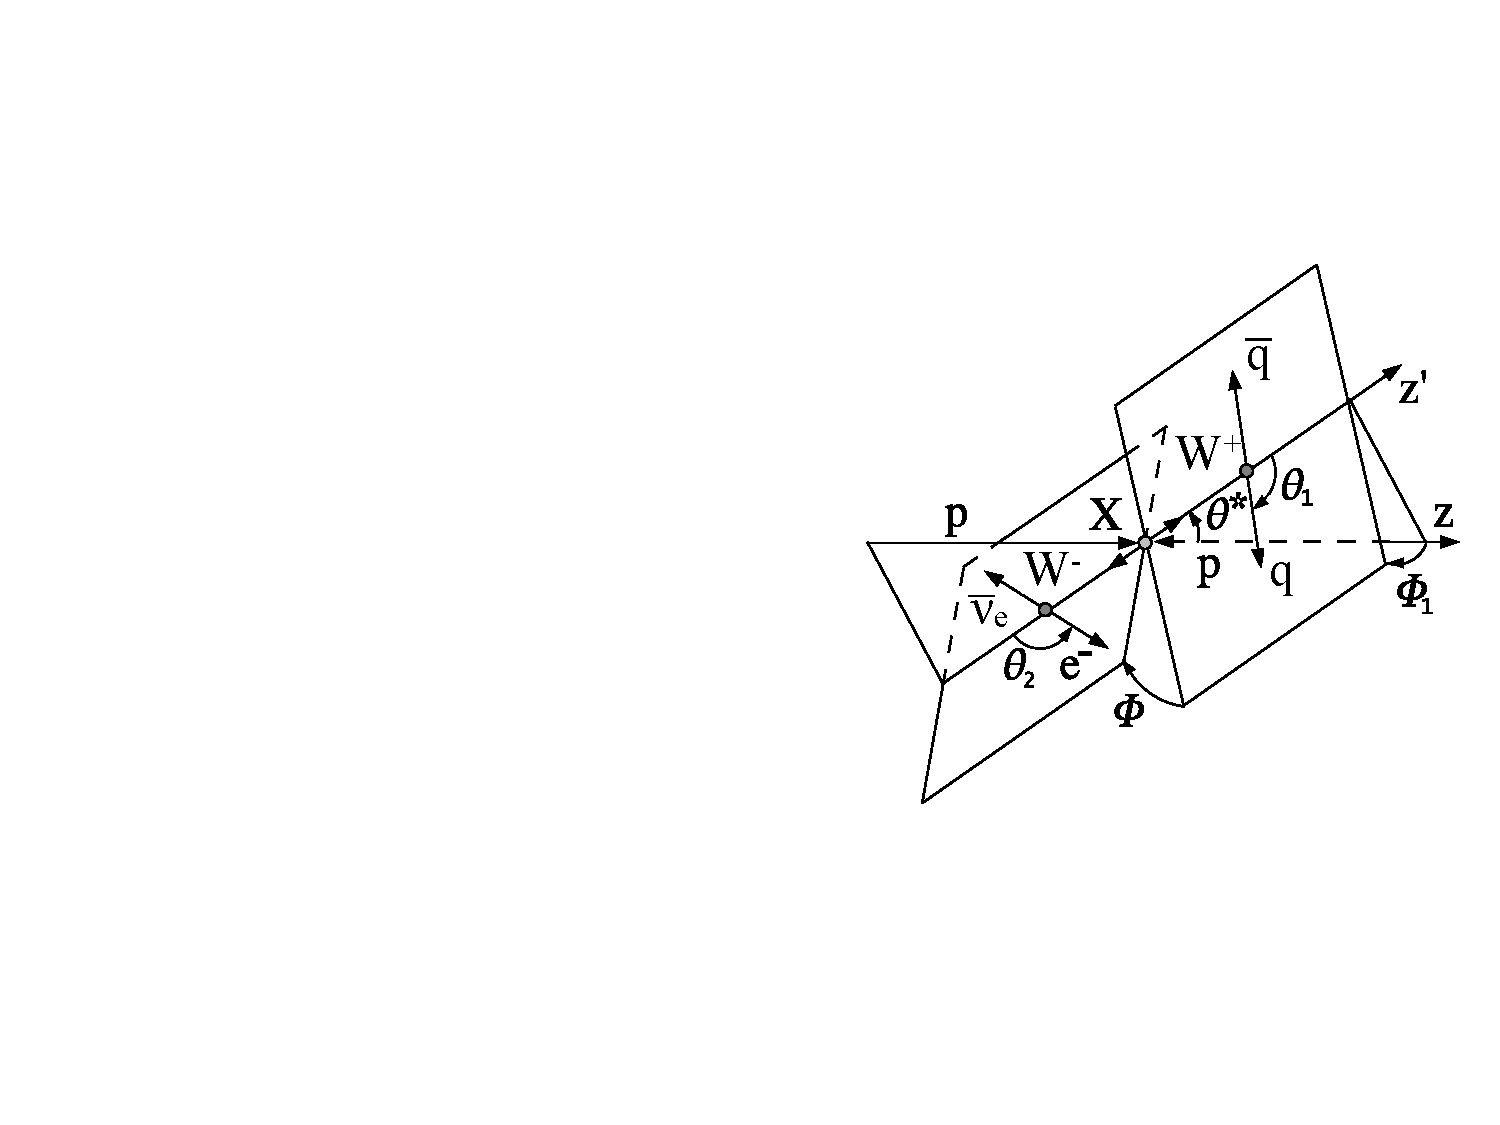
\includegraphics[width=0.5\textwidth]{plots/anaexample/angles_wwlvjj.pdf}
  \caption{\label{fig:anglesWWlvjj}Angular definition for the $WW\to l\nu jj$ process}
\end{figure}
%%%%%%%%%%%%%%%%%%%
The angle $\cos\theta^{\ast}$ is the polar angle between the parton collision axis z and the $X$ 
decay axis $z'$, both defined in the $X$ rest frame. The angle $\Phi_1$ is the azimuthal angle
between the $zz'$ plane and the decay plane of hadronic $W$. The angles 
$\cos\theta^{\ast}$ and $\Phi_1$ are denoted as production
angles because they depend on the production mechanism, $gg$ or $q\bar{q}$.
For the SM Higgs which is a spin-zero particle, the production angles are flat (before acceptance). 
The angle $\Phi$ is the angle between the decay planes of the two $W$ systems in the $X$ rest
frame. The angle $\theta_i$ is the angle between
the direction of the fermion f from $W \to f\bar{f}$ and the direction opposite the $X$ in
the $W_i$ rest frame, where index i = 1, 2 refers to the first or second $W$ boson. 
In the case of the $\cos\theta_i$ angle from the hadronic $W$, it is ambiguous as to which jet is originating from the 
fermion or anti-fermion, so the angles is defined from $0$ to $\pi$ for the leading $p_T$ jet.  
Finally, The angles $\Phi$, $\cos\theta_1$ and $\cos\theta_2$ do not depend on the production mechanism and are denoted as the helicity angles.

The observables $m_{l\nu jj}$ and $m_{jj}$ are excluded from the MVA inputs.
The observable, $m_{l\nu jj}$, is not used because it is the distribution of this observable which is used
in the extraction of the upper limit.
The observable, $m_{jj}$, is not used since the $m_{jj}$ distribution is used to extract from the sideband to the signal region
to extract a data-driven shape for the background in the $m_{l\nu jj}$ spectrum. 
The leaves the five angular variables as inputs to the multivariate discriminant.  
As an example, the related search for the Higgs in the $ZZ \to 2l2q$ final state at CMS~\cite{CMS2l2q} uses these five observables
in an angular discriminant. 
Since the invariant masses are not used in the multivariate discriminant, the angular variables are defined in a loose window in 
$m_{l\nu jj}$ in order to take into account the correlations between the angles and the masses.  

In addition, to the five angular variables the $p_T$ of the WW system $p_{T,WW}$ 
and longitudinal boost (rapidity) $Y_{WW}$ are also used.  
The $Y_{WW}$ distribution comes from the parton distribution functions. 
The $p_{T,WW}$ distribution comes from next-to-leading order effects.  
The lepton charge is also included to give some discrimination power since the $W$ + jets background 
is asymmetric with respect to charge while the SM Higgs signal will be symmetric in lepton charge.  
These two quantities in addition to the mass and angular quantities form a full set of kinematic observables for process.
Other discriminating observables such as the $p_T$ of the $W\to jj$ system are not independent of the full set 
(and particularly of $m_{l\nu jj}$ and $m_{jj}$) are thus not used since they can sculpt the invariant mass distributions
to make the background more "signal-like".

Combining all the inputs together the final set of inputs to the multivariate discriminant is:
\begin{equation}
\{ \cos\theta_1, \cos\theta_2, \Phi, \cos\theta^{\ast}, \Phi_1, p_{T,WW}, Y_{WW}, {\rm lepton~charge} \}.
\end{equation}
%As an example, we plot the input variables for the SM Higgs mass of 300~GeV for the 2-jet $W\to\mu\nu$ category in Fig.~\ref{fig:inputs3002jmu}.

The MVA discriminant is optimized with a training, 
within a mass window around each nominal Higgs mass.
The mass window is defined by means of a gaussian fit on the signal peak, 
to be the nominal mass $\pm~1\sigma$.
The performance of the three classifiers studied -- linear discriminant, 
likelihood, and boosted decision tree -- have been compared, 
and since the likelihood gives the best discrimination, 
it has been chosen for our analysis.

The discriminant is exploited by means of a single cut on it, chosen
for each of the working points separately, on the basis of a scan over
a range of MVA cut values at discrete intervals. The figure of merit
was chosen to be the expected median exclusion limit achieved for the
cut value based on the same limit setup described in
Section~\ref{sec:limitExtraction} and a reasonable assumption on the
systematics. The results in all cases revealed an optimum cut value
that minimized the expected limit with a resolution better than a
tenth of the signal strength excluded.

The technical details of the optimization are described in the CMS analysis note AN-2012/008. %FIXME citation needed

\subsection{MVA validation}

As an example for the SM Higgs mass of 400~GeV for the 2-jet $W\to\mu\nu$ category, 
we plot the input variables in Fig.~\ref{fig:inputs4002jmu}. 
The left plot in Figure~\ref{fig:datamcplot:mva2j400mu} 
shows the data-MC comparison for MVA output: 
the agreement is good in the region of phase space where the cuts are made, 
and in general in the whole range where there is signal. 
As a further test,
the output of the MVA has been looked at in a ttbar-enriched sample,
selected by requiring exactly four jets in the event,
two of which b-tagged and two of which anti-btagged.
These latter are taken as the hadronic $W$ decay products.
The MVA output in data and MC is shown on the righthand side of Figure~\ref{fig:datamcplot:mva2j400mu} 
and the agreement is reasonable at high MVA values where the Higgs
sits.
The same distributions are shown as an example for a low Higgs mass working point, 
in the same Figure.
The 2-jet $W\to{}e\nu$ case is reported.
In this case, the agreement of the MVA shape in the analysis phase space is less good,
while the one in the ttbar-enriched region,
which is expected to be closer to the signal topology in terms of physics objects,
is good.

\begin{figure}[ht]
  \centering
  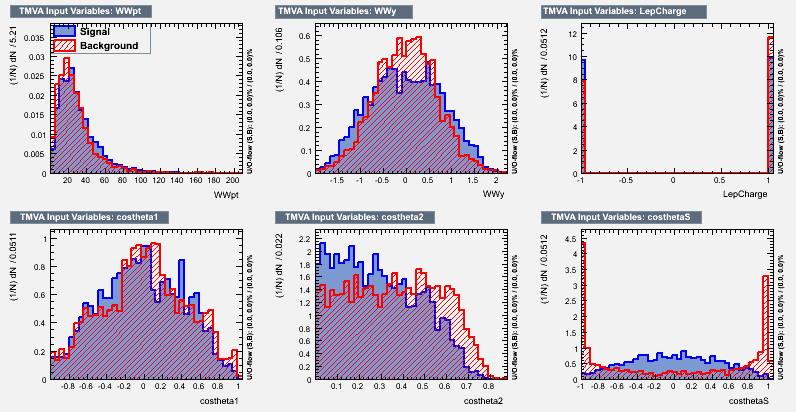
\includegraphics[width=0.8\textwidth]{plots/anaexample/TMVA_350_nJ2_mu_variables_id_c1.png}
  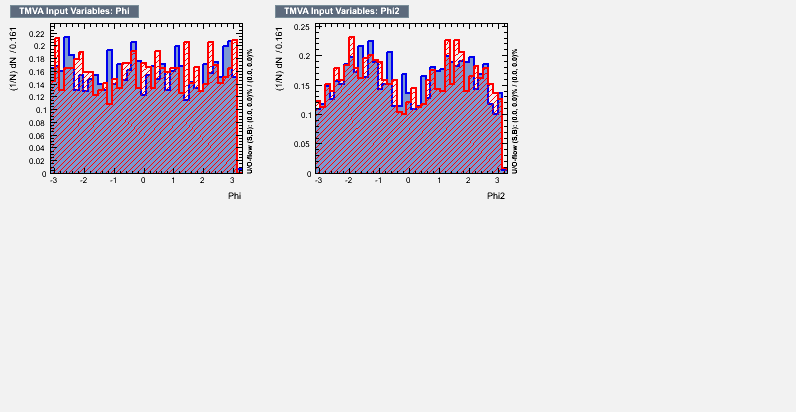
\includegraphics[width=0.8\textwidth]{plots/anaexample/TMVA_350_nJ2_mu_variables_id_c2.png}	
  \caption{\label{fig:inputs4002jmu}Inputs to the multivariate discriminant for SM Higgs mass of 350~GeV for the 2-jet $W\to\mu\nu$ category}
\end{figure}

\begin{figure}[ht]
  \centering
  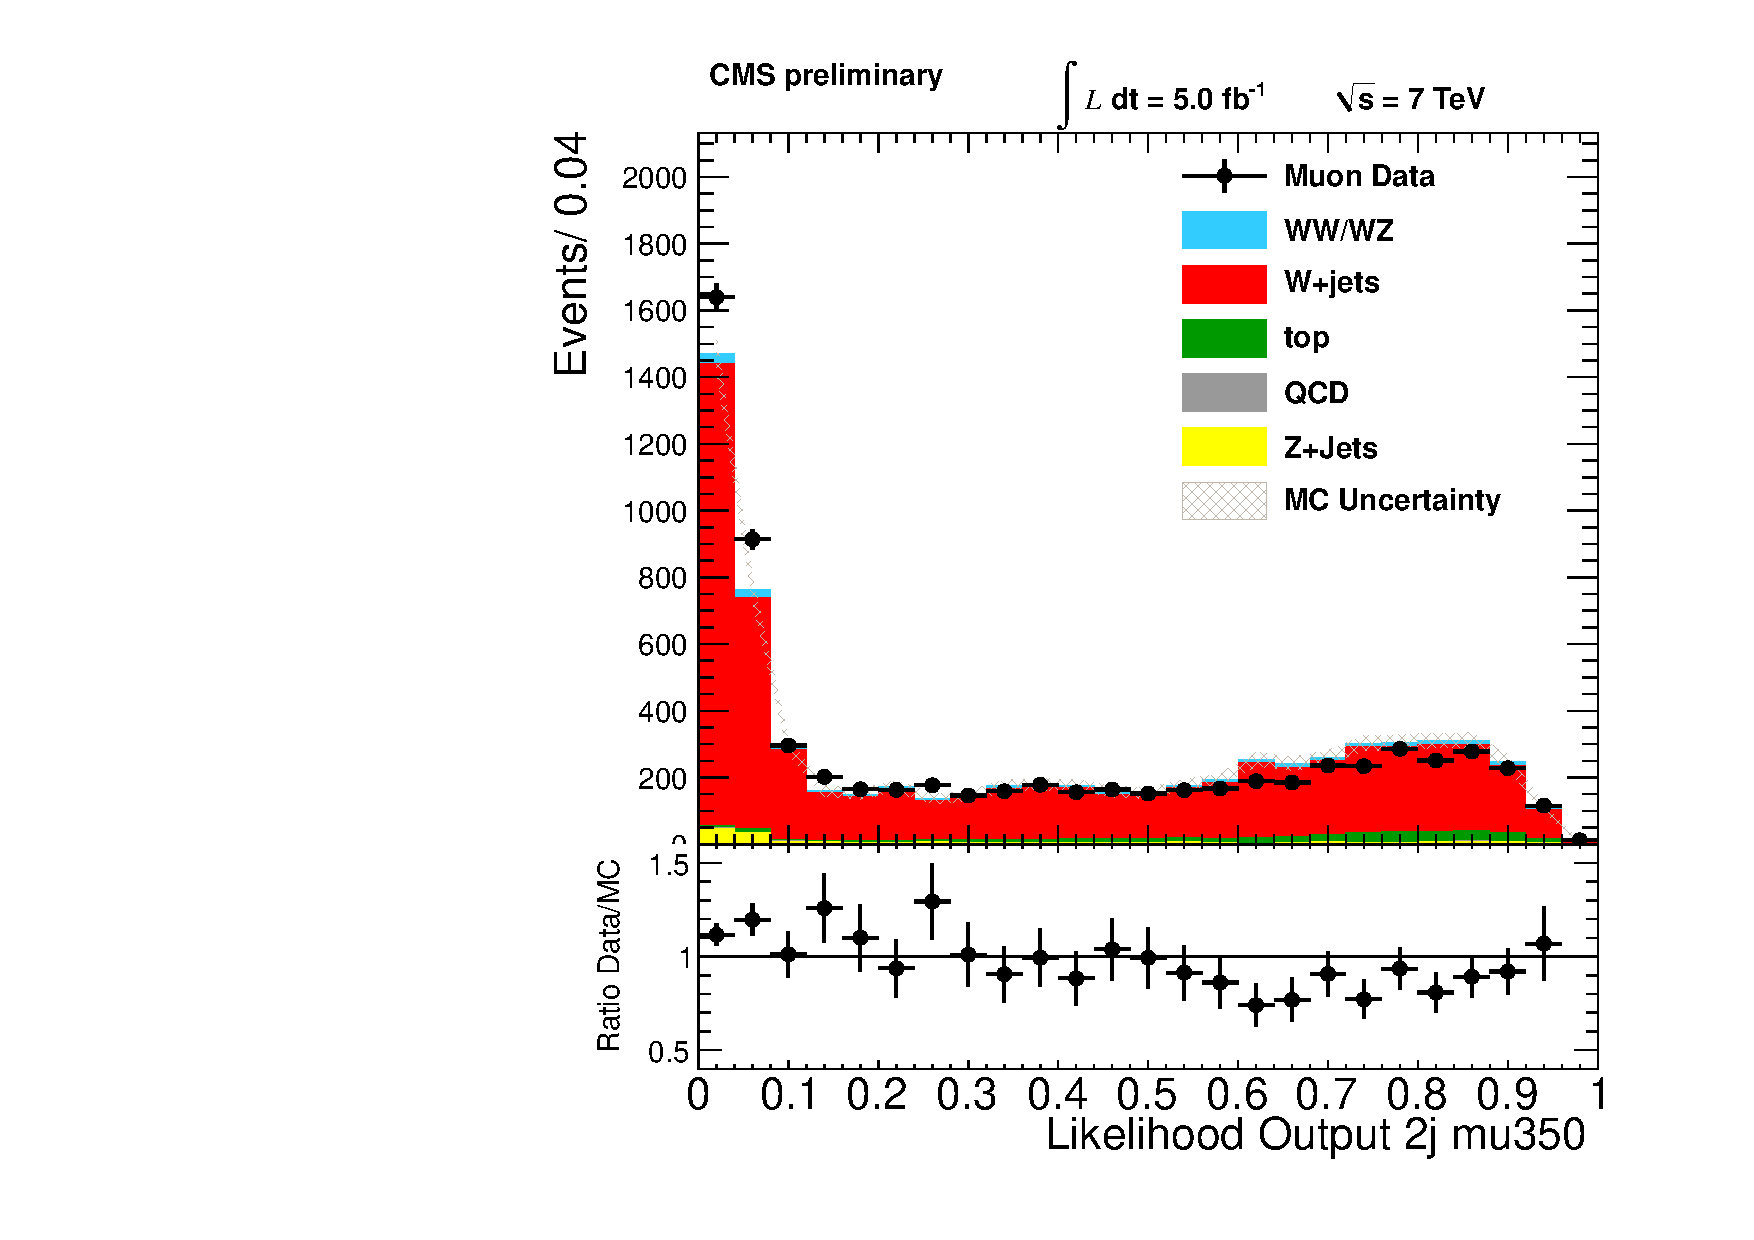
\includegraphics[width=0.49\textwidth]{plots/anaexample/cl-mva2j350mu-normal.pdf}
  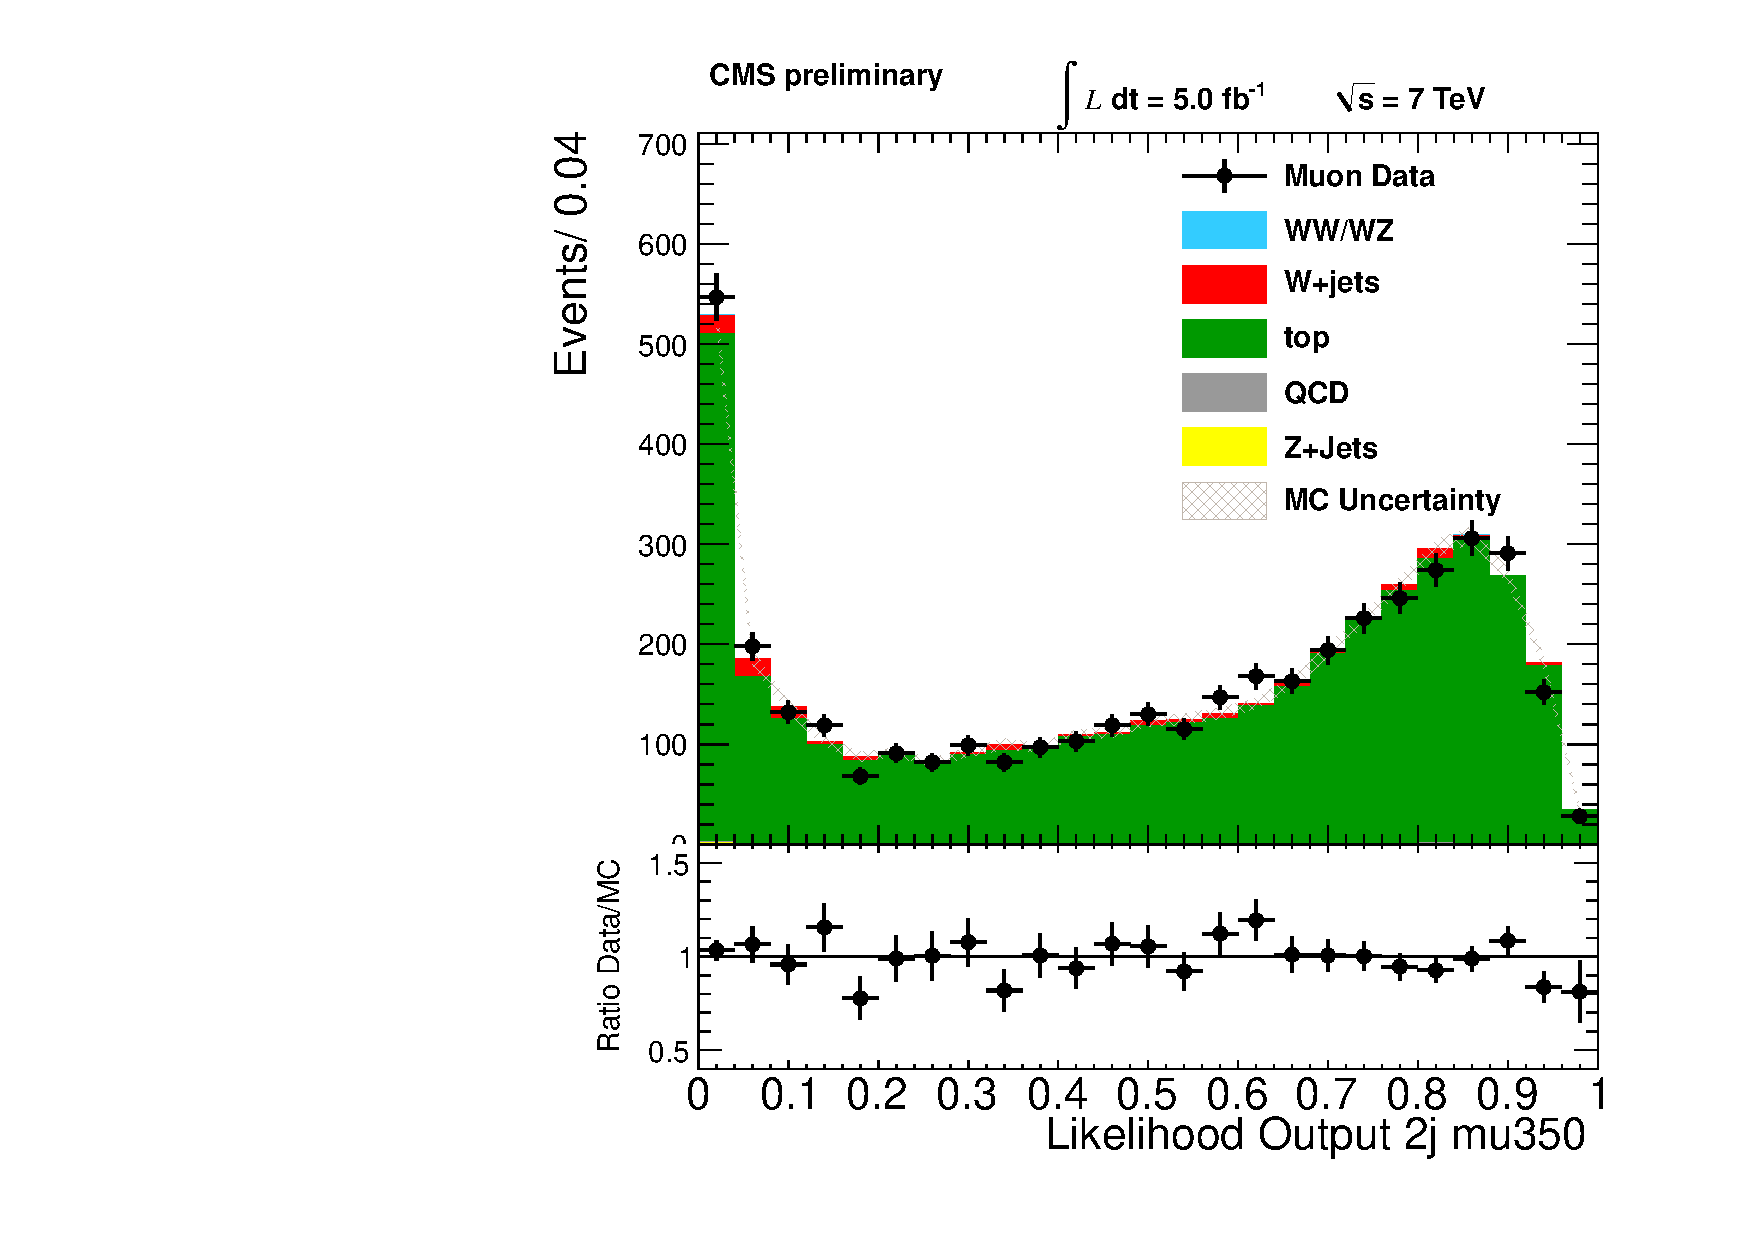
\includegraphics[width=0.49\textwidth]{plots/anaexample/cl-mva2j350mu-inTTbar.pdf}
  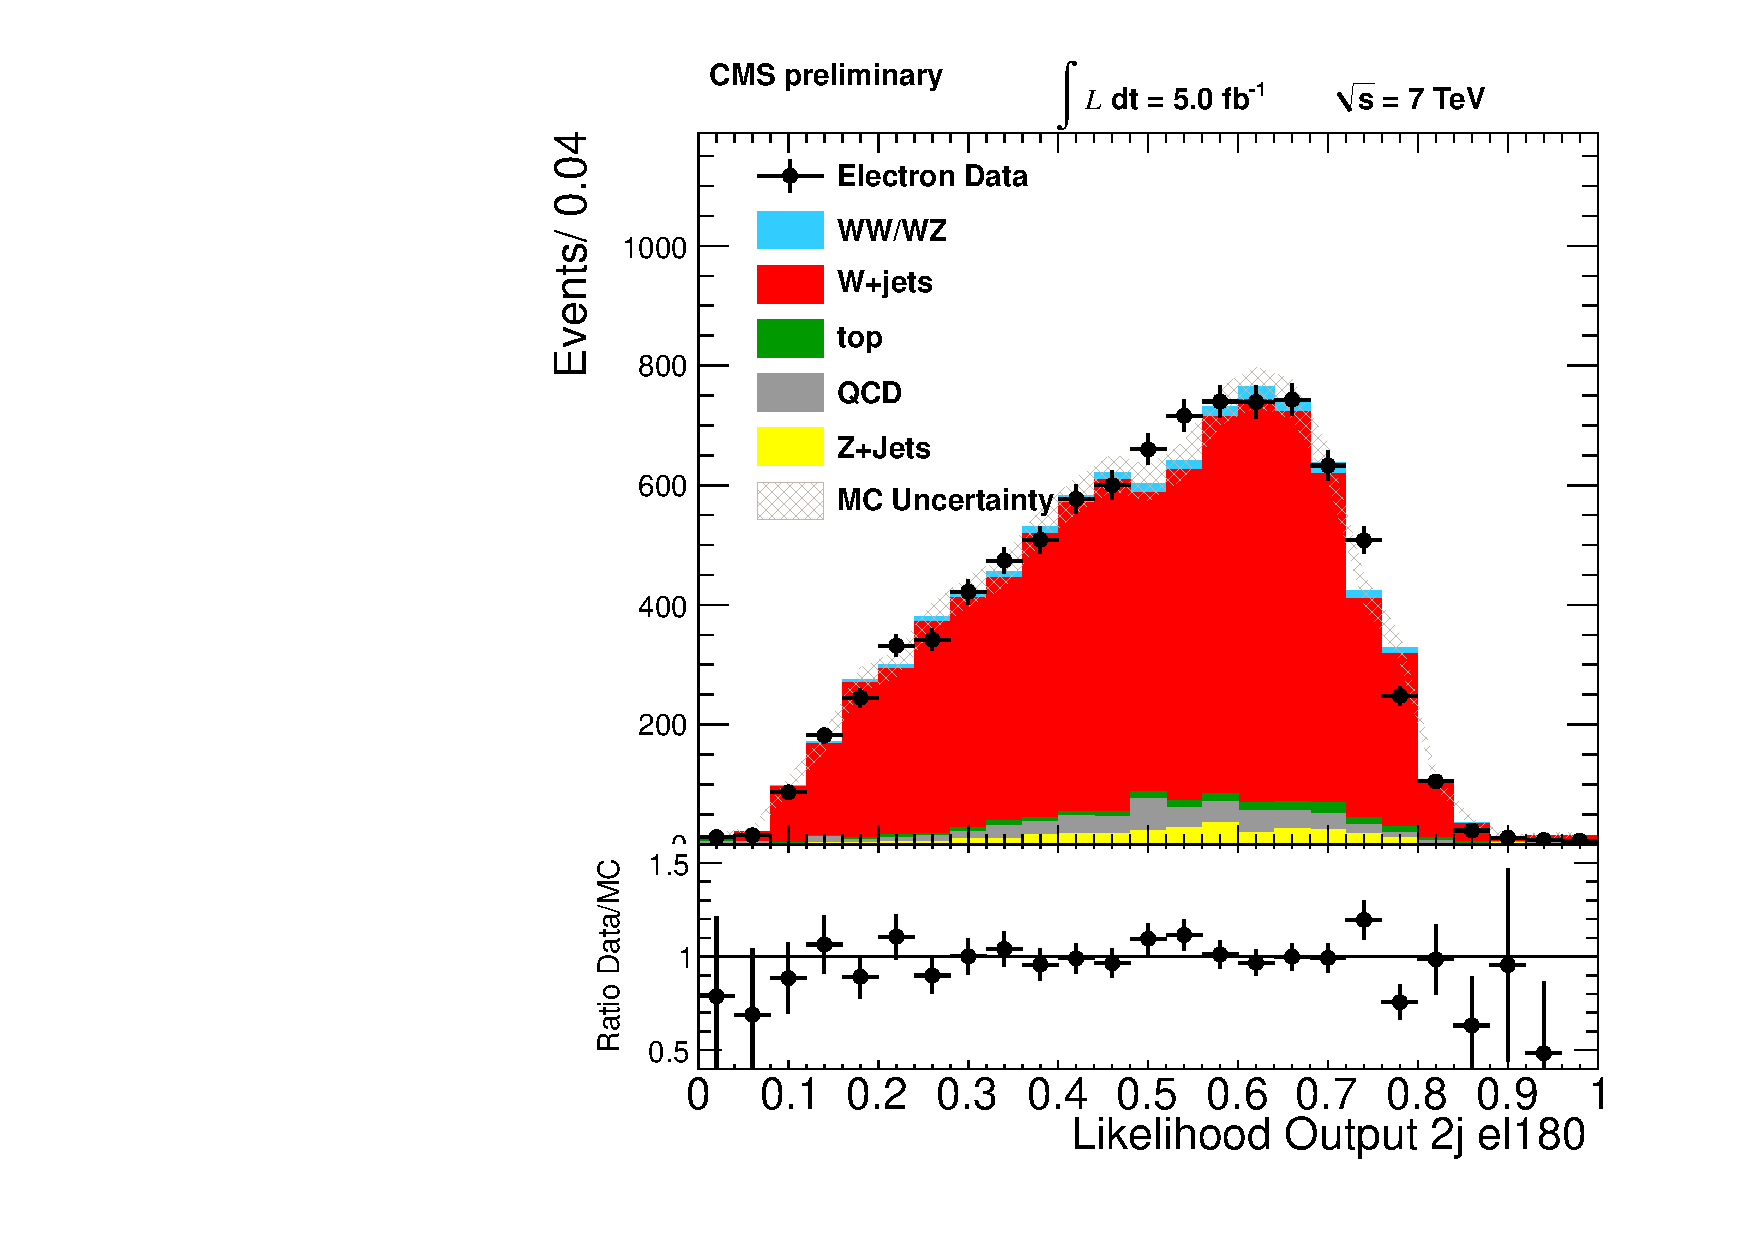
\includegraphics[width=0.49\textwidth]{plots/anaexample/cl-mva2j180el-normal.pdf}
  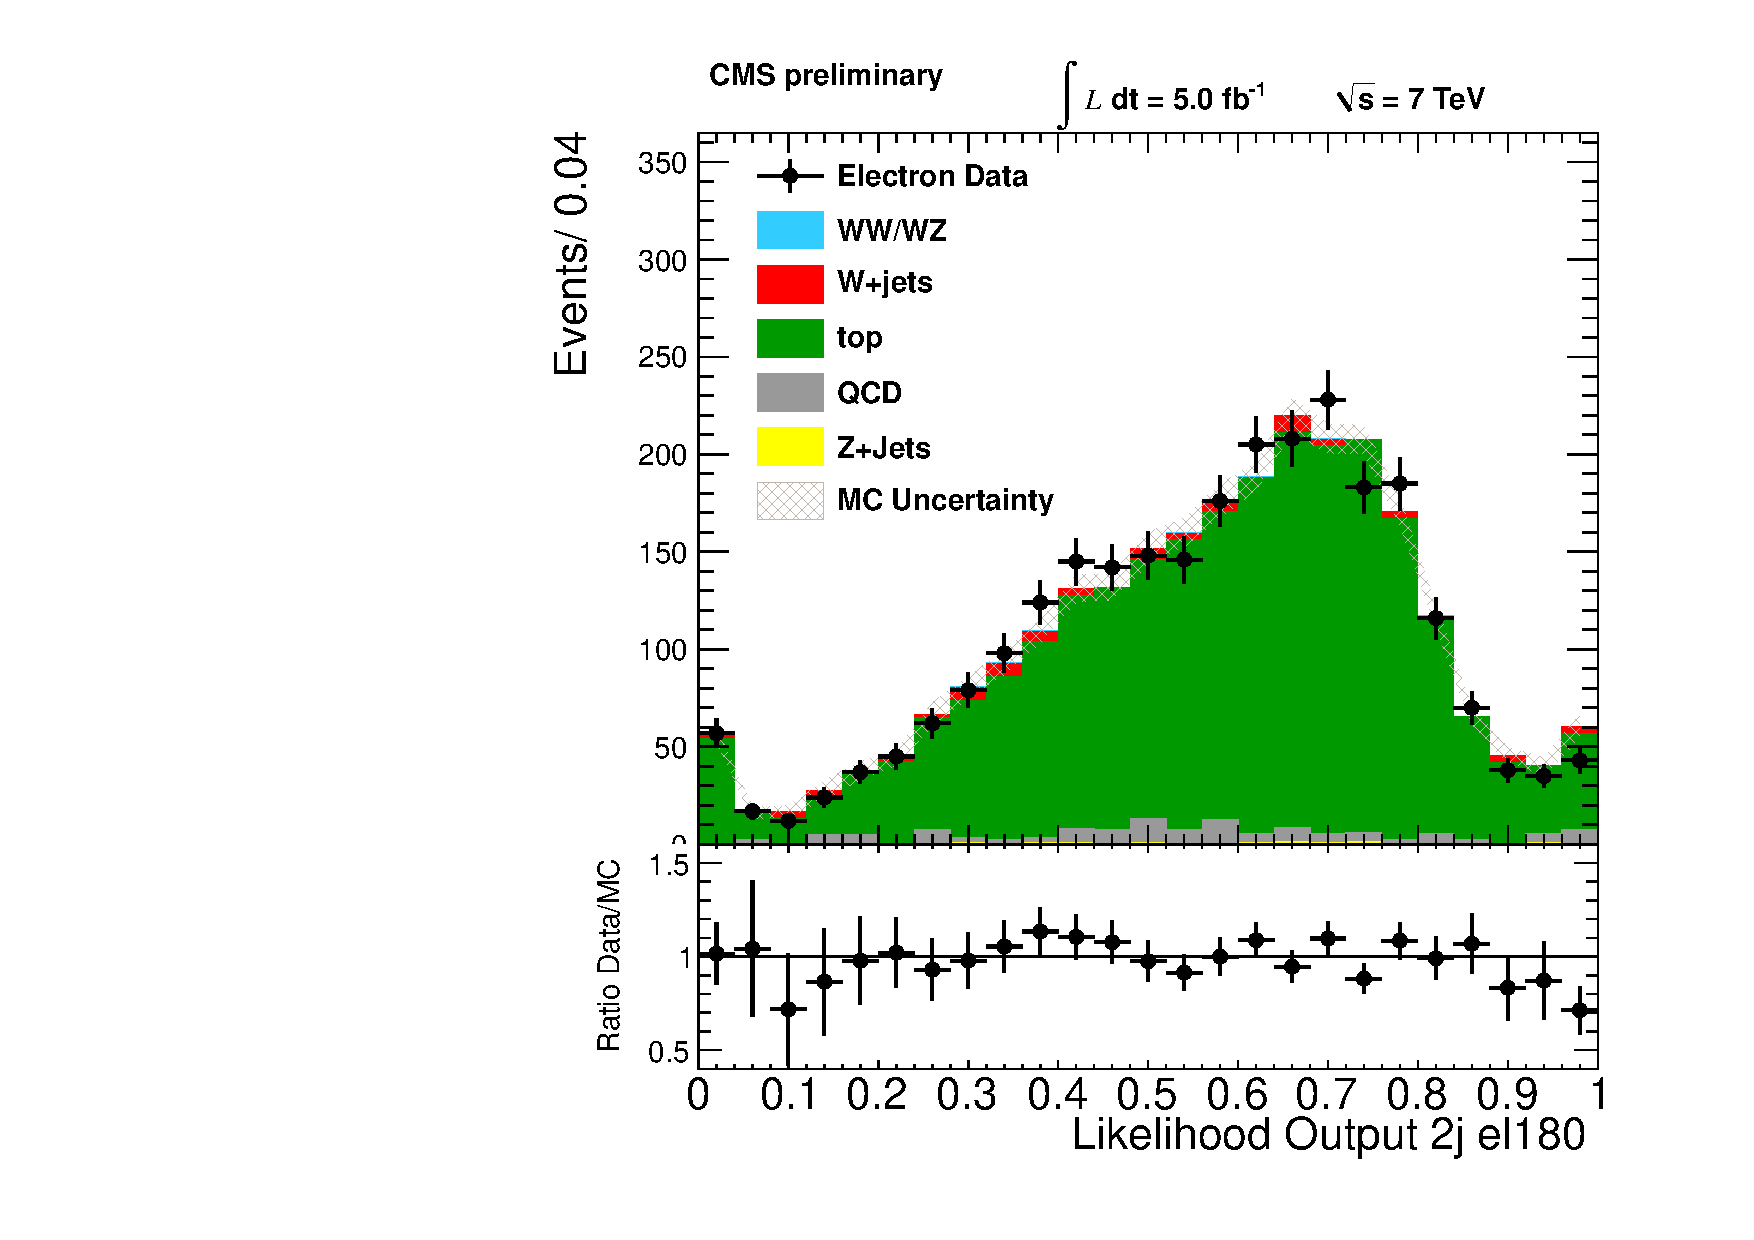
\includegraphics[width=0.49\textwidth]{plots/anaexample/cl-mva2j180el-inTTbar.pdf}
  \caption{Data-MC comparison of MVA output
    for the SM Higgs mass of 350~GeV for the 2-jet $W\to\mu\nu$ category (top)
    and for 180~GeV for the 2-jet $W\to{}e\nu$ one (bottom). 
    The left plot is after the standard event selection 
    and the right plot in a ttbar enriched sample. 
    MC samples are normalized to the integrated luminosity.}
  \label{fig:datamcplot:mva2j400mu}    
\end{figure}

\subsection{Quark-gluon likelihood discriminant}

The quark-gluon likelihood discriminant gives a measure of the
likelihood of a jet originating from a quark or gluon~\cite{qgAN}.  At
leading order, the SM Higgs signal consists of quark-originated jets
while the background is an admixture of both quark- and
gluon-originated jets.  To discriminate signal events from background
events, one may calculate the likelihood for each jet in the event and
apply an optimized cut. We chose to apply a cut based on quark-gluon
likelihood simultaneously with but separately from the MVA cut.

A brief inspection of the quark-gluon likelihood distributions for
signal versus background across the various mass points indicates that
the most performant discriminating variable appears to be the
likelihood derived for the sub-leading jet, $\mathcal{L}_{qg,2}$,
particularly at high mass (Fig.~\ref{fig:qgld}). To optimize the cut
value, a scan was performed over discrete cut values in a way
analogous to the MVA cut optimization procedure described above,
except in this case the optimal MVA cut was applied first. The optimal
cut value for $\mathcal{L}_{qg,2}$ was chosen based on the best
expected limit derived after the cut. It was determined that a benefit
was to be gained by applying a cut on $\mathcal{L}_{qg,2}$ only for
mass points $\ge$500~GeV.

\begin{figure}[ht]
  \centering
  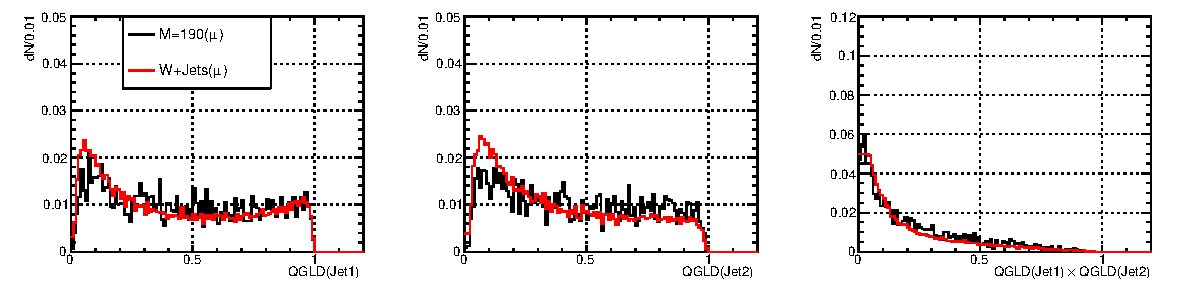
\includegraphics[width=0.9\textwidth]{plots/anaexample/qgldm190mu.pdf}
  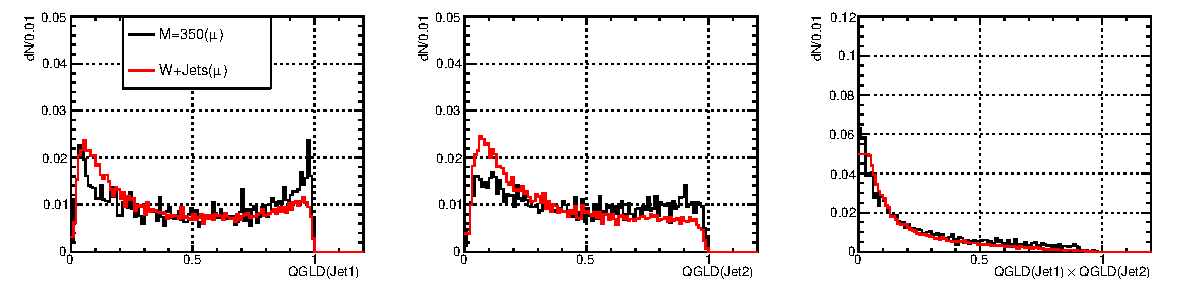
\includegraphics[width=0.9\textwidth]{plots/anaexample/qgldm350mu.pdf}
  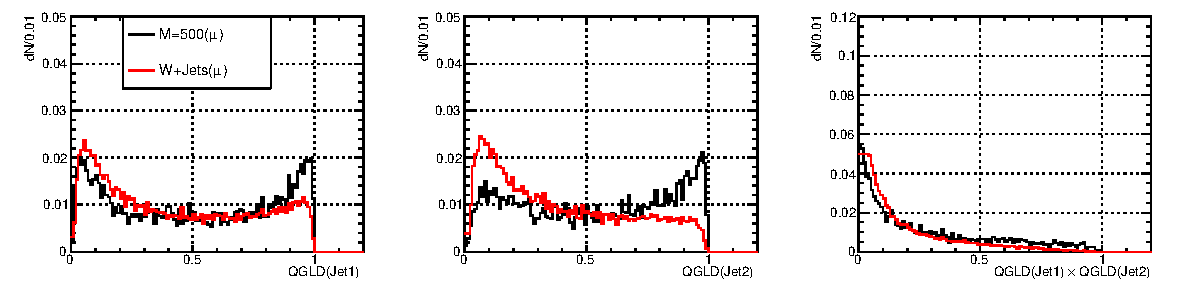
\includegraphics[width=0.9\textwidth]{plots/anaexample/qgldm500mu.pdf}
  \caption{Plots of the quark-gluon likelihood discriminant for the
    leading and subleading jets, and their product, for three signal
    mass points and W+jets background.}
  \label{fig:qgld}    
\end{figure}
